\documentclass{article}
\usepackage{graphicx} %package to manage images
\usepackage[utf8]{inputenc}
\usepackage[a4paper, total={6in, 8in}]{geometry}
\usepackage{float}
\usepackage{xurl}
\title{Relatório 7 \\ Análise de transições}
\author{Pedro A. S. O. Neto}
\date{Abril, 2022}

\begin{document}

\maketitle

\section{Cronograma}

O cronograma abaixo representa 12 mêses de trabalho. A linha cinza representa o mês atual.

\begin{figure}[H]
\noindent\makebox[\textwidth]{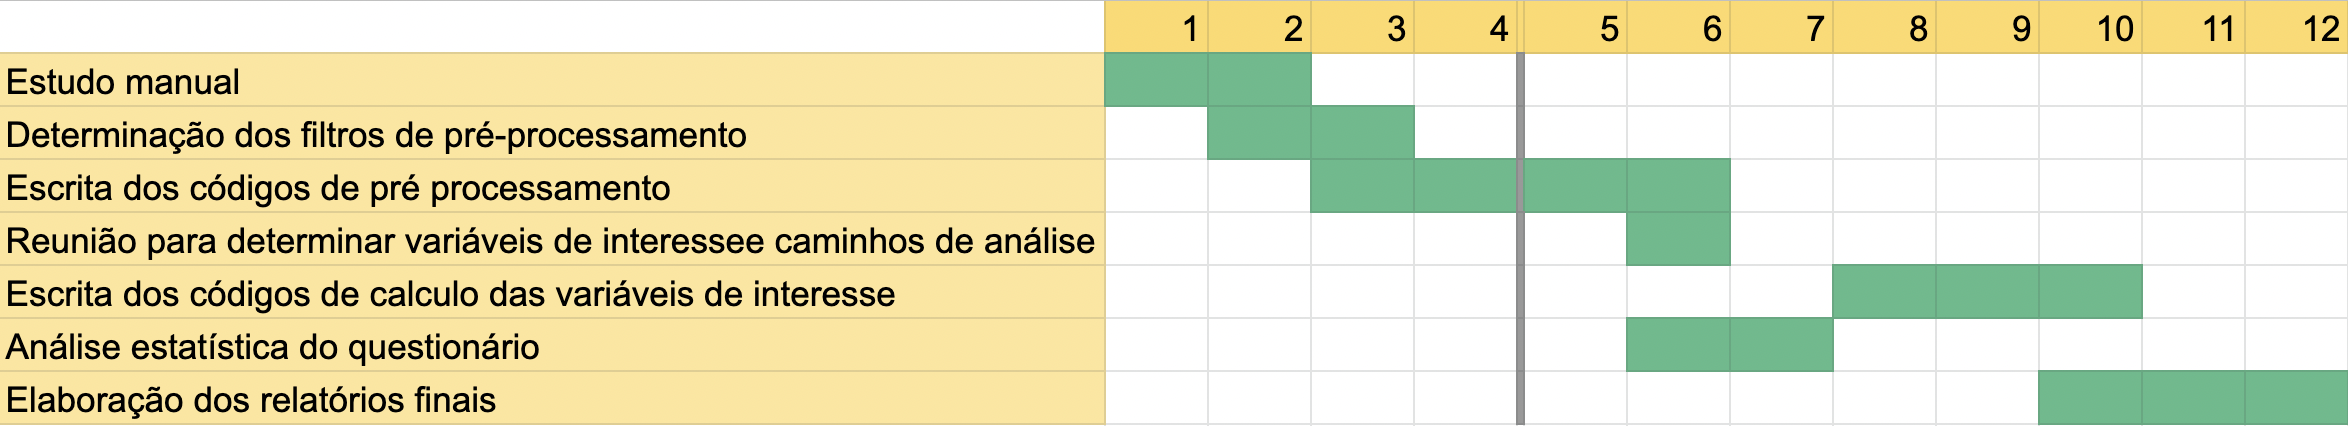
\includegraphics[width=0.9\paperwidth]{"./cronogram.png"}}
\end{figure}

\end{document}


